\chapter{Wheatstone Bridge}

\section{Aim}
To learn how to use a Wheatstone bridge to determine the resistance of an unknown resistor

\section{Background Information}
A Wheatstone bridge is a special electronic circuit which can be used in larger circuits for different purposes. However, one of its functions can be to determine the resistance of an unknown resistor very precisely. It has certain advantageous over other ohmmeters including an independence of variations in the voltage in the circuit. Thus, it is important to learn how to use a Wheatstone bridge properly. We will learn how to construct a Wheatstone bridge circuit by using a meter bridge. 

\section{Materials}
2-3 Batteries (1.5 V size D), switch, standard resistor (2$\Omega$), 5 unknown resistors\slash resistance wire of different lengths, galvanometer, meter bridge, connecting wires

\section{Procedure}
\begin{enumerate}
\item Construct the circuit depicted where $R$ is a standard resistor and $S$ is an unknown resistor or a resistance wire. 
\item Slide the jockey of the galvanometer across the meter bridge until you find a point where no current flows through the galvanometer. Measure the distances $L_1$ and $L_2$. 
\item Repeat step (2) four more times by replacing resistor $R$ with other resistors $R_2-R_5$ or four different lengths of resistance wire.
\item Tabulate your results.
\end{enumerate}

\begin{figure}[h!]
\centering
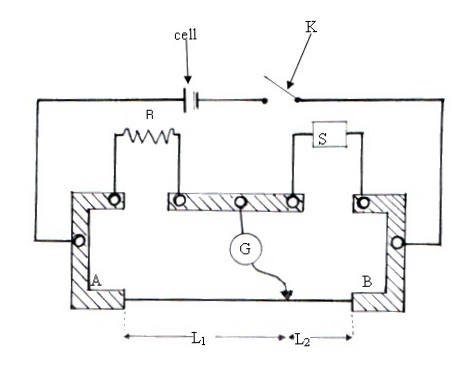
\includegraphics[width=12cm]{./img/wheatstone-bridge-1.jpg}
\caption{Wheatstone Bridge practical setup}
\label{fig:wheatstone-bridge-1}
\end{figure}

\section{Analysis and Interpretation}
\begin{enumerate}
\item We know that the resistance of a segment of the wire on the meter bridge is proportional to what?
\item When the galvanometer in a Wheatstone bridge shows no deflection, what does it mean?
\item When a Wheatstone bridge is balanced, the ratio of the unknown resistor and the standard resistor equals the ratio of the resistance of segment 2 and segment 1 of the meter bridge. Use this equation to construct an equation which relates the unknown resistor $R$ to the resistance of the standard resistor $S$ and the two lengths $L_1$ and $L_2$.
\item What are the resistances of the unknown resistors?
\end{enumerate}

\section{Conclusion}
Explain how to use a Wheatstone bridge to determine the resistance of an unknown resistor. 

\section{Questions for Discussion}
\begin{enumerate}
\item What are the sources of error in this activity?
\item Why should the wires connecting the unknown resistor and the Wheatstone bridge be as short as possible?
\item Create a new relation which relates the resistance of the unknown resistor with the standard resistor $R$ and $L_1$ without $L_2$.
\item Is it possible to repeat the experiment with the positions of the standard resistor and the unknown resistor switched in the Wheatstone bridge? 
\item Could you construct the Wheatstone bridge without using a meter bridge? Explain.
\item Could this experiment be used to determine the resistivity of a conductor?
\end{enumerate}

\section{Reflection and Self Assessment}
\begin{enumerate}
\item Is there anything you do not understand in this activity? If so, what is it and in what ways can you increase your understanding?
\item Did you have difficulties setting up this activity? If so what where they and what can you do next time to avoid these difficulties?
\end{enumerate}